% Title: glps_renderer figure
% Creator: GL2PS 1.3.8, (C) 1999-2012 C. Geuzaine
% For: Octave
% CreationDate: Sat Mar  3 15:12:24 2018
\setlength{\unitlength}{1pt}
\begin{picture}(0,0)
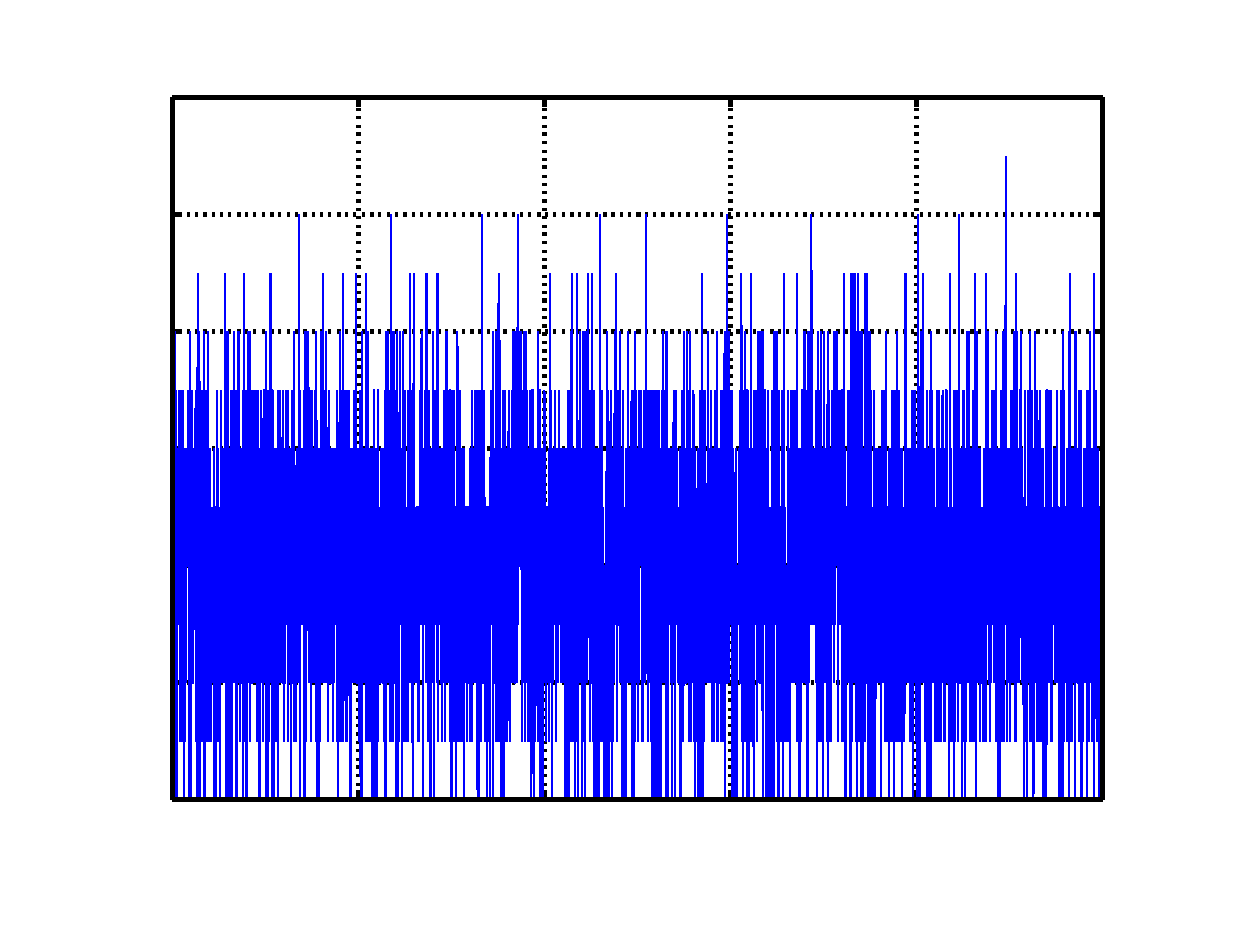
\includegraphics{disp_waypoints-inc}
\end{picture}%
\begin{picture}(576,432)(0,0)
\fontsize{18}{0}
\selectfont\put(74.88,50.9933){\makebox(0,0)[t]{\textcolor[rgb]{0,0,0}{{0}}}}
\fontsize{18}{0}
\selectfont\put(164.16,50.9933){\makebox(0,0)[t]{\textcolor[rgb]{0,0,0}{{1000}}}}
\fontsize{18}{0}
\selectfont\put(253.44,50.9933){\makebox(0,0)[t]{\textcolor[rgb]{0,0,0}{{2000}}}}
\fontsize{18}{0}
\selectfont\put(342.72,50.9933){\makebox(0,0)[t]{\textcolor[rgb]{0,0,0}{{3000}}}}
\fontsize{18}{0}
\selectfont\put(432,50.9933){\makebox(0,0)[t]{\textcolor[rgb]{0,0,0}{{4000}}}}
\fontsize{18}{0}
\selectfont\put(521.28,50.9933){\makebox(0,0)[t]{\textcolor[rgb]{0,0,0}{{5000}}}}
\fontsize{18}{0}
\selectfont\put(69.8755,55.9934){\makebox(0,0)[r]{\textcolor[rgb]{0,0,0}{{0}}}}
\fontsize{18}{0}
\selectfont\put(69.8755,112.161){\makebox(0,0)[r]{\textcolor[rgb]{0,0,0}{{2}}}}
\fontsize{18}{0}
\selectfont\put(69.8755,168.329){\makebox(0,0)[r]{\textcolor[rgb]{0,0,0}{{4}}}}
\fontsize{18}{0}
\selectfont\put(69.8755,224.497){\makebox(0,0)[r]{\textcolor[rgb]{0,0,0}{{6}}}}
\fontsize{18}{0}
\selectfont\put(69.8755,280.664){\makebox(0,0)[r]{\textcolor[rgb]{0,0,0}{{8}}}}
\fontsize{18}{0}
\selectfont\put(69.8755,336.832){\makebox(0,0)[r]{\textcolor[rgb]{0,0,0}{{10}}}}
\fontsize{18}{0}
\selectfont\put(69.8755,393){\makebox(0,0)[r]{\textcolor[rgb]{0,0,0}{{12}}}}
\fontsize{24}{0}
\selectfont\put(298.08,28.9933){\makebox(0,0)[t]{\textcolor[rgb]{0,0,0}{{Amostra}}}}
\fontsize{24}{0}
\selectfont\put(43.8755,224.497){\rotatebox{90}{\makebox(0,0)[b]{\textcolor[rgb]{0,0,0}{{Quantidade [un]}}}}}
\fontsize{24}{0}
\selectfont\put(298.08,403){\makebox(0,0)[b]{\textcolor[rgb]{0,0,0}{{Dispersão do número de pontos de passagem gerados}}}}
\end{picture}
